\documentclass[11pt]{article}
\usepackage[margin=1in]{geometry}
\usepackage{longtable}
\usepackage{float}
\usepackage[bitheight=5ex]{bytefield}
\usepackage{color}
\usepackage{amsmath,tikz,drawstack}
\usepackage[bookmarksopen=true]{hyperref}
\usetikzlibrary{fit,shapes,positioning,matrix}
\usetikzlibrary{arrows,chains}
\usetikzlibrary{decorations.pathreplacing}

\definecolor{lightcyan}{rgb}{0.84,1,1}
\definecolor{lightgreen}{rgb}{0.64,1,0.71}
\definecolor{lightred}{rgb}{1,0.7,0.71}
\definecolor{namecolor}{RGB}{105,139,34}
\definecolor{elemcolor}{RGB}{234,232,170}

\newcommand{\colorbitbox}[3]{%
\rlap{\bitbox{#2}{\color{#1}\rule{\width}{\height}}}%
\bitbox{#2}{#3}}

\title{Bootloader implementation guide on ST platform(nand boot)}
\author{Liu Yanqiang}
\date{\today}

\begin{document}
\sloppy
\maketitle

\setcounter{section}{0}
\section{Compents for the bootloader}
	There are four compents for the bootloader to bootup the system:
	\begin{itemize}
		\item xLoader

				xLoader is the first piece code excuted by the CPU after powerup, it must
				set the CPU clock, init DDR, read ApLoader from NAND or SDCARD and then
				jump to ApLoader.
				
				The xLoader is copied from nand to the internal RAM by the Boot ROM after 
				powerup, and its size must be less than 14KiB.

		\item ApLoader

				ApLoader is the second part of the bootloader, it may be copied to the DDR 
				by the xLoader from nand or from SDCARD, depends on the startup conditions.
				The ApLoader must load the logo show for LCD, init the rear camera, load os
				image to DDR, setup boot params for OS and jump to OS.

				The ApLoader's size is usally less than NAND block size(128KiB)
				
		\item splash.rgb

				This compent is binary format of a picture, the ApLoader will read it to the
				DDR for LCD to show it on the screen.

				The size of this file is depends on the screen size and data format the LCD
				controller used. If we use RGB565, and the screen resolution is 480x272, the
				size of this file will be about 256KiB.

		\item os image

				OS image is an excutable image, the ApLoader will load it to DDR from NAND and
				jump the the entry to the OS.

				The size of the OS image is usally between 3MiB to 5MiB.
	\end{itemize}

\section{NAND layout for bootloader and OS}
	In order to get stable system performance, we must back up these compents, and design
	reasonable strategy to use these backups.

	The Boot ROM will read only the first block for NAND boot, if the first block is bad or
	the data in it is broken, the system will not boot, and simply hungup. So we don't need
	to backup the xLoader.

	This is the layout of all the four compents with backups in NAND:

\begin{figure}[H]
	\begin{center}
	\begin{bytefield}[bitwidth=9em]{4}
		\bitbox[b]{1}{$\overbrace{\hspace{8em}}^\text{one block(256KiB)}$} \\
		\begin{rightwordgroup}{Total 15MiB}
		\colorbitbox{namecolor}{1}{xLoader}			&
		\colorbitbox{elemcolor}{1}{ApLoader}		&
		\colorbitbox{elemcolor}{1}{ApLoader}		&
		\colorbitbox{elemcolor}{1}{ApLoader}		\\
		\colorbitbox{elemcolor}{1}{ApLoader}		&
		\colorbitbox{elemcolor}{1}{ApLoader}		&
		\colorbitbox{elemcolor}{1}{ApLoader}		&
		\colorbitbox{elemcolor}{1}{ApLoader}		\\
		\colorbitbox{lightcyan}{1}{splash.rgb}		&
		\colorbitbox{lightcyan}{1}{splash.rgb}		&
		\colorbitbox{lightcyan}{1}{splash.rgb}		&
		\colorbitbox{lightcyan}{1}{splash.rgb}		\\
		\colorbitbox{lightgreen}{4}{OS Image Copy 1}	\\
		\colorbitbox{lightgreen}{4}{OS Image Copy 1}	\\
		\colorbitbox{lightgreen}{4}{OS Image Copy 1}	\\
		\colorbitbox{lightgreen}{4}{OS Image Copy 1}	\\
		\colorbitbox{lightgreen}{4}{OS Image Copy 1}	\\
		\colorbitbox{lightgreen}{4}{OS Image Copy 1}	\\
		\colorbitbox{lightred}{4}{OS Image Copy 2}	\\
		\colorbitbox{lightred}{4}{OS Image Copy 2}	\\
		\colorbitbox{lightred}{4}{OS Image Copy 2}	\\
		\colorbitbox{lightred}{4}{OS Image Copy 2}	\\
		\colorbitbox{lightred}{4}{OS Image Copy 2}	\\
		\colorbitbox{lightred}{4}{OS Image Copy 2}	
		\end{rightwordgroup}
	\end{bytefield}
	\begin{footnotesize}
	\begin{longtable}[l]{llp{0.5\textwidth}}
	Image Name	&	Copies			& NAND space			\\
	xLoader		&	1 copy.			& 0x00000000~0x00040000 \\
	ApLoader	&	7 copies.		& 0x00040000~0x00200000 \\
	splash.rgb	&	4 copies.		& 0x00200000~0x00300000 \\
	OS image 1	&	1 copy.			& 0x00300000~0x00900000 \\
	OS image 2	&	1 copy.			& 0x00900000~0x00F00000 
	\end{longtable}
	\end{footnotesize}
	\caption{Bootloader compents layout in NAND}
	\end{center}
\end{figure}

	If the first block of the nand is bad, the system can not boot.

	For the ApLoader and splash.rgb, if bad blocks found in their area, the copies for
	the compents will be less than this picture displayed. For example, if block 2 of
	the nand is bad, the ApLoader will have only 6 copies. 

	If bad blocks found in the OS area, we just skip these blocks. The total size of the
	OS image must be smaller than 6MiB. However, if one bad block found in this area, the
	OS maxsize must be limited to 5.75MiB.

\section{Images layout}
	We must add checksums to these images in order to make sure we get the correct data
	from nand. This layout format is applied both in nand and for files to be used by
	the programmer. That is to say, we must process the origin images with special PC
	tools to get the images which can be used to be flashed to nand.

	The image layout for all the compents are like this:
	
\begin{figure}[H]
\tikzset{
    datastruct/.style={
		rectangle, rounded corners, rectangle split,
		rectangle split part align={center,left},
		rectangle split part fill={namecolor,elemcolor},draw
	}
}
\begin{tikzpicture}
	\matrix (imagestruct) [block,text width=16mm] {
 		& & & & \\
	};

	\node[draw,fit=(imagestruct-1-1),block nodes,fill=namecolor]{image header};
	\node[draw,fit=(imagestruct-1-2)(imagestruct-1-5),block nodes,fill=elemcolor]{image contents};
	\draw [black,decorate,decoration={brace,amplitude=10pt}] (imagestruct-1-1.north west) -- (imagestruct-1-1.north east) node [black,midway,above=4pt,xshift=-2pt] {SUB\_PAGE\_SIZE(512)};
	\draw [black,decorate,decoration={brace,mirror,amplitude=10pt}] (imagestruct-1-1.south west) -- (imagestruct-1-1.south east) node (imageheaders) [midway,below=4pt] {};
	\draw [black,decorate,decoration={brace,mirror,amplitude=10pt}] (imagestruct-1-1.south east) -- (imagestruct-1-5.south east) node (imagecontents) [midway,below=4pt] {};

	% header struct
	\node[datastruct, rectangle split parts=4,below=of imagestruct-1-1] (imageheadert) {
		\nodepart{one}
		image\_header\_t
		\nodepart{two}
		uint32\_t magic;
		\nodepart{three}
		uint32\_t length;
		\nodepart{four}
		uint32\_t crc;
	};

	\draw [black,decorate,decoration={brace,amplitude=10pt}] (imageheadert.north west) -- (imageheadert.north east) node (imageheaderd) [midway,above=4pt] {};

	% connect elements
	\draw [->] (imageheaders) -- (imageheaderd);
	\draw [<-] (imagecontents) |- (imageheadert.three east);
	\draw [<-] (imagecontents) |- (imageheadert.four east);
\end{tikzpicture}

	\begin{footnotesize}
	\begin{longtable}[l]{llp{0.5\textwidth}}
	Image Name	&	Magic			\\
	xLoader		&	0xA5A58000		\\
	ApLoader	&	0xA5A58001		\\
	splash.rgb	&	0xA5A58002		\\
	OS image 	&	0xA5A58006			
	\end{longtable}
	\end{footnotesize}
\caption{Compents image layout}
\end{figure}

	For ApLoader, splash.rgb and OS image, we can write the file get from SD card directly to
	the nand, because the PC tool has add the image header to the origin images. But for xLoader,
	we can't write the header to the nand, only the image contents, because the Boot Rom can't
	recongnize our image headers.

\section{xLoader flow chart}
	xLoader is the first piece of code excuted by the CPU after reset. The Boot Rom will copy it
	from the first nand block to the internal RAM, at address 0xA000\_0000. The code must copy
	itself to 0xA000\_4800, then excute the rest code.

	This is the detailed flow chart of xLoader:

\begin{figure}[H]
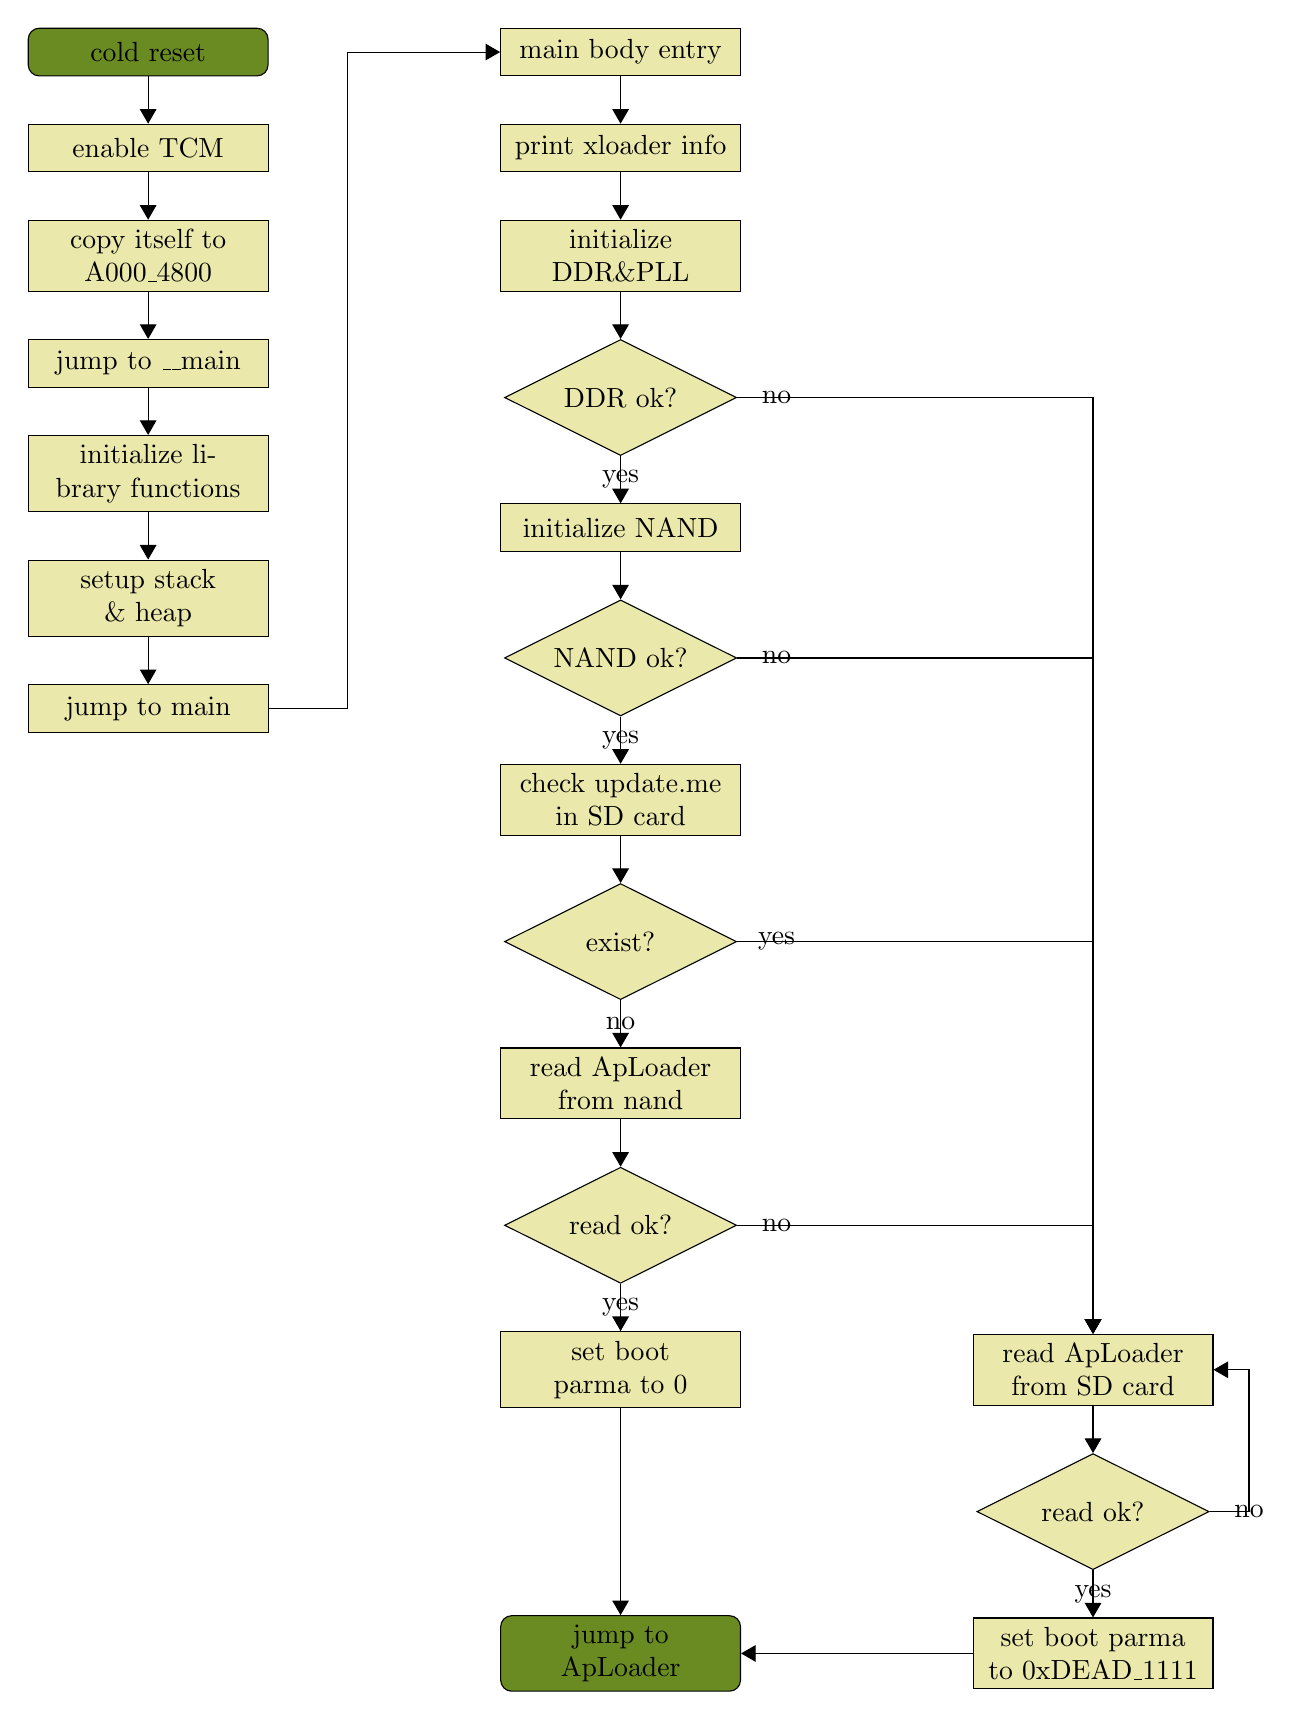
\begin{tikzpicture}[%
    >=triangle 60,              % Nice arrows; your taste may be different
    start chain=going below,    % General flow is top-to-bottom
    node distance=6mm and 60mm, % Global setup of box spacing
    every join/.style={norm},   % Default linetype for connecting boxes
    ]
\tikzset{
  base/.style={draw, on chain, on grid, align=center, minimum height=4ex},
  proc/.style={base, rectangle, text width=8em, fill=elemcolor},
  test/.style={base, diamond, aspect=2, text width=5em, fill=elemcolor},
  term/.style={base, rectangle, text width=8em, rounded corners, fill=namecolor},
}

\node [term] (p0) {cold reset};
\node [proc] (p1) {enable TCM};	
\node [proc] (p2) {copy itself to A000\_4800};	
\node [proc] (p3) {jump to \_\_main};	
\node [proc] (p4) {initialize library functions};	
\node [proc] (p5) {setup stack \& heap};	
\node [proc] (p6) {jump to main};	

\node [proc,right=of p0] (p7) {main body entry};
\node [proc] (p8) {print xloader info};
\node [proc] (p9) {initialize DDR\&PLL};
\node [test] (p10) {DDR ok?};
\node [proc] (p11) {initialize NAND};
\node [test] (p12) {NAND ok?};
\node [proc] (p13) {check update.me in SD card};
\node [test] (p14) {exist?};
\node [proc] (p15) {read ApLoader from nand};
\node [test] (p16) {read ok?};
\node [proc] (p17) {set boot parma to 0};

\node [proc,right=of p17] (p18) {read ApLoader from SD card};
\node [test] (p19) {read ok?};
\node [proc] (p20) {set boot parma to 0xDEAD\_1111};
\node [term,left=of p20] (p21) {jump to ApLoader};

\draw [->] (p0.south) -- (p1.north);
\draw [->] (p1.south) -- (p2.north);
\draw [->] (p2.south) -- (p3.north);
\draw [->] (p3.south) -- (p4.north);
\draw [->] (p4.south) -- (p5.north);
\draw [->] (p5.south) -- (p6.north);

\draw [->] (p6.east) -- ++(right:10mm) |- (p7.west);
\draw [->] (p7.south) -- (p8.north);
\draw [->] (p8.south) -- (p9.north);
\draw [->] (p9.south) -- (p10.north);
\draw [->] (p10.south) -- node {yes} (p11.north);
\draw [->] (p10.east) -- ++(right:5mm) node {no} -| (p18.north);
\draw [->] (p11.south) -- (p12.north);
\draw [->] (p12.south) -- node {yes} (p13.north);
\draw [->] (p12.east) -- ++(right:5mm) node {no} -| (p18.north);
\draw [->] (p13.south) -- (p14.north);
\draw [->] (p14.south) -- node {no} (p15.north);
\draw [->] (p14.east) -- ++(right:5mm) node {yes} -| (p18.north);
\draw [->] (p15.south) -- (p16.north);
\draw [->] (p16.south) -- node {yes} (p17.north);
\draw [->] (p16.east) -- ++(right:5mm) node {no} -| (p18.north);
\draw [->] (p17.south) -- (p21.north);

\draw [->] (p18.south) -- (p19.north);
\draw [->] (p19.south) -- node {yes} (p20.north);
\draw [->] (p19.east) -- ++(right:5mm) node {no} |- (p18.east);
\draw [->] (p20.west) -- (p21.east);

\end{tikzpicture}
	\begin{footnotesize}
	\begin{longtable}[l]{llp{0.5\textwidth}}
	BOOT PARAM		&	APLOADER ACTION						\\
	0x0000\_0000	&	Read image from nand and boot.		\\
	0xDEAD\_XXXX	&	Recovery the system from sdcard.
	\end{longtable}
	\end{footnotesize}
\caption{xLoader flow chart}
\end{figure}

	The xLoader code size is less than 14KiB, it doesn't use the DDR, it just initialize the
	DDR for ApLoader. The xLoader use the internal SRAM for code and stack. This is the resource
	used by xLoader:
\begin{footnotesize}
\begin{longtable}[l]{llp{0.5\textwidth}}
SPACE							& USAGE						\\
0xA000\_4800 to 0xA000\_8000	& xLoader code				\\
0xFFFE\_3B00 to 0xFFFE\_4000	& Stack						\\
0xFFFE\_2000 to 0xFFFE\_3B00	& Heap						
\end{longtable}
\end{footnotesize}

\section{ApLoader flow chart}
	The xLoader copies ApLoader to the DDR either from NAND or from external SD card, then
	jumps to ApLoader. Figure 4 is the flow chart of the ApLoader.

\begin{figure}[H]
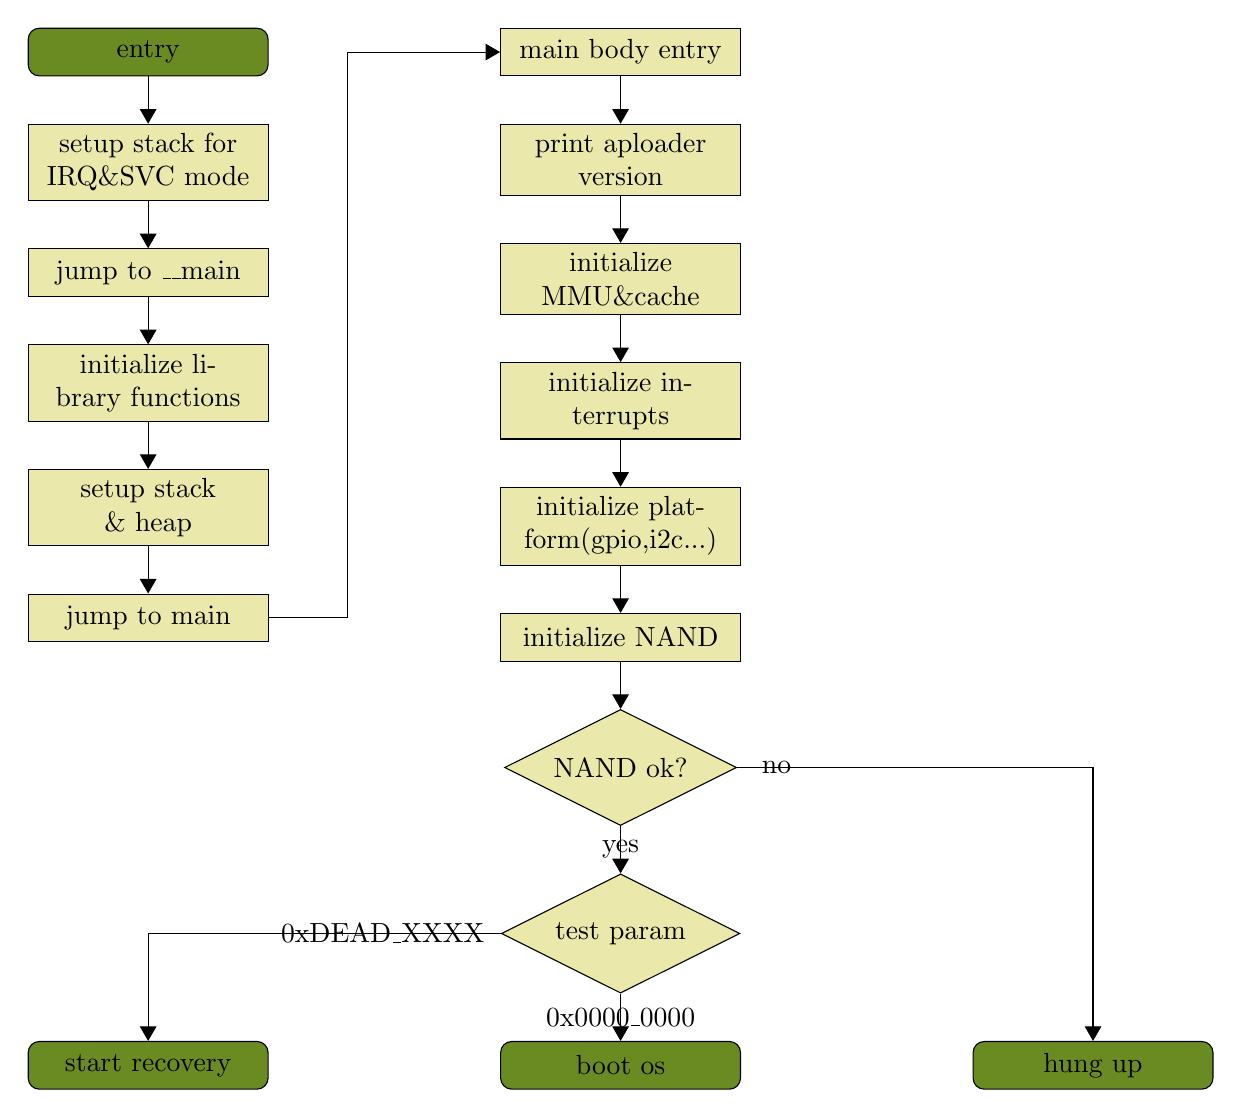
\begin{tikzpicture}[%
    >=triangle 60,              % Nice arrows; your taste may be different
    start chain=going below,    % General flow is top-to-bottom
    node distance=6mm and 60mm, % Global setup of box spacing
    every join/.style={norm},   % Default linetype for connecting boxes
    ]
\tikzset{
  base/.style={draw, on chain, on grid, align=center, minimum height=4ex},
  proc/.style={base, rectangle, text width=8em, fill=elemcolor},
  test/.style={base, diamond, aspect=2, text width=5em, fill=elemcolor},
  term/.style={base, rectangle, text width=8em, rounded corners, fill=namecolor},
}

\node [term] (p0) {entry};
\node [proc] (p1) {setup stack for IRQ\&SVC mode};
\node [proc] (p2) {jump to \_\_main};
\node [proc] (p3) {initialize library functions};	
\node [proc] (p4) {setup stack \& heap};	
\node [proc] (p5) {jump to main};	

\node [proc,right=of p0] (p6) {main body entry};
\node [proc] (p7) {print aploader version};
\node [proc] (p8) {initialize MMU\&cache};
\node [proc] (p9) {initialize interrupts};
\node [proc] (p10) {initialize platform(gpio,i2c...)};
\node [proc] (p11) {initialize NAND};
\node [test] (p12) {NAND ok?};
\node [test] (p13) {test param};

\node [term] (p14) {boot os};
\node [term,left=of p14] (p15) {start recovery};

\node [term,right=of p14] (p16) {hung up};

% connect
\draw [->] (p0.south) -- (p1.north);
\draw [->] (p1.south) -- (p2.north);
\draw [->] (p2.south) -- (p3.north);
\draw [->] (p3.south) -- (p4.north);
\draw [->] (p4.south) -- (p5.north);
\draw [->] (p5.east) -- ++(right:10mm) |- (p6.west);

\draw [->] (p6.south) -- (p7.north);
\draw [->] (p7.south) -- (p8.north);
\draw [->] (p8.south) -- (p9.north);
\draw [->] (p9.south) -- (p10.north);
\draw [->] (p10.south) -- (p11.north);
\draw [->] (p11.south) -- (p12.north);
\draw [->] (p12.south) -- node {yes} (p13.north);
\draw [->] (p12.east) -- ++(right:5mm) node {no} -| (p16.north);
\draw [->] (p13.south) -- node {0x0000\_0000} (p14.north);
\draw [->] (p13.west) -- ++(left:15mm) node {0xDEAD\_XXXX} -| (p15.north);

\end{tikzpicture}
\caption{ApLoader flow chart}
\end{figure}

	The ApLoader has two main functions, one is to boot the os at normal conditions,
	the other is to recovery the system when debug or upgrade needded. Figure 4 only
	shows the entry for boot os and recovery.

\subsection{The recovery process}
	Figure 5 is the process of recovery.

\begin{figure}[H]
\begin{center}
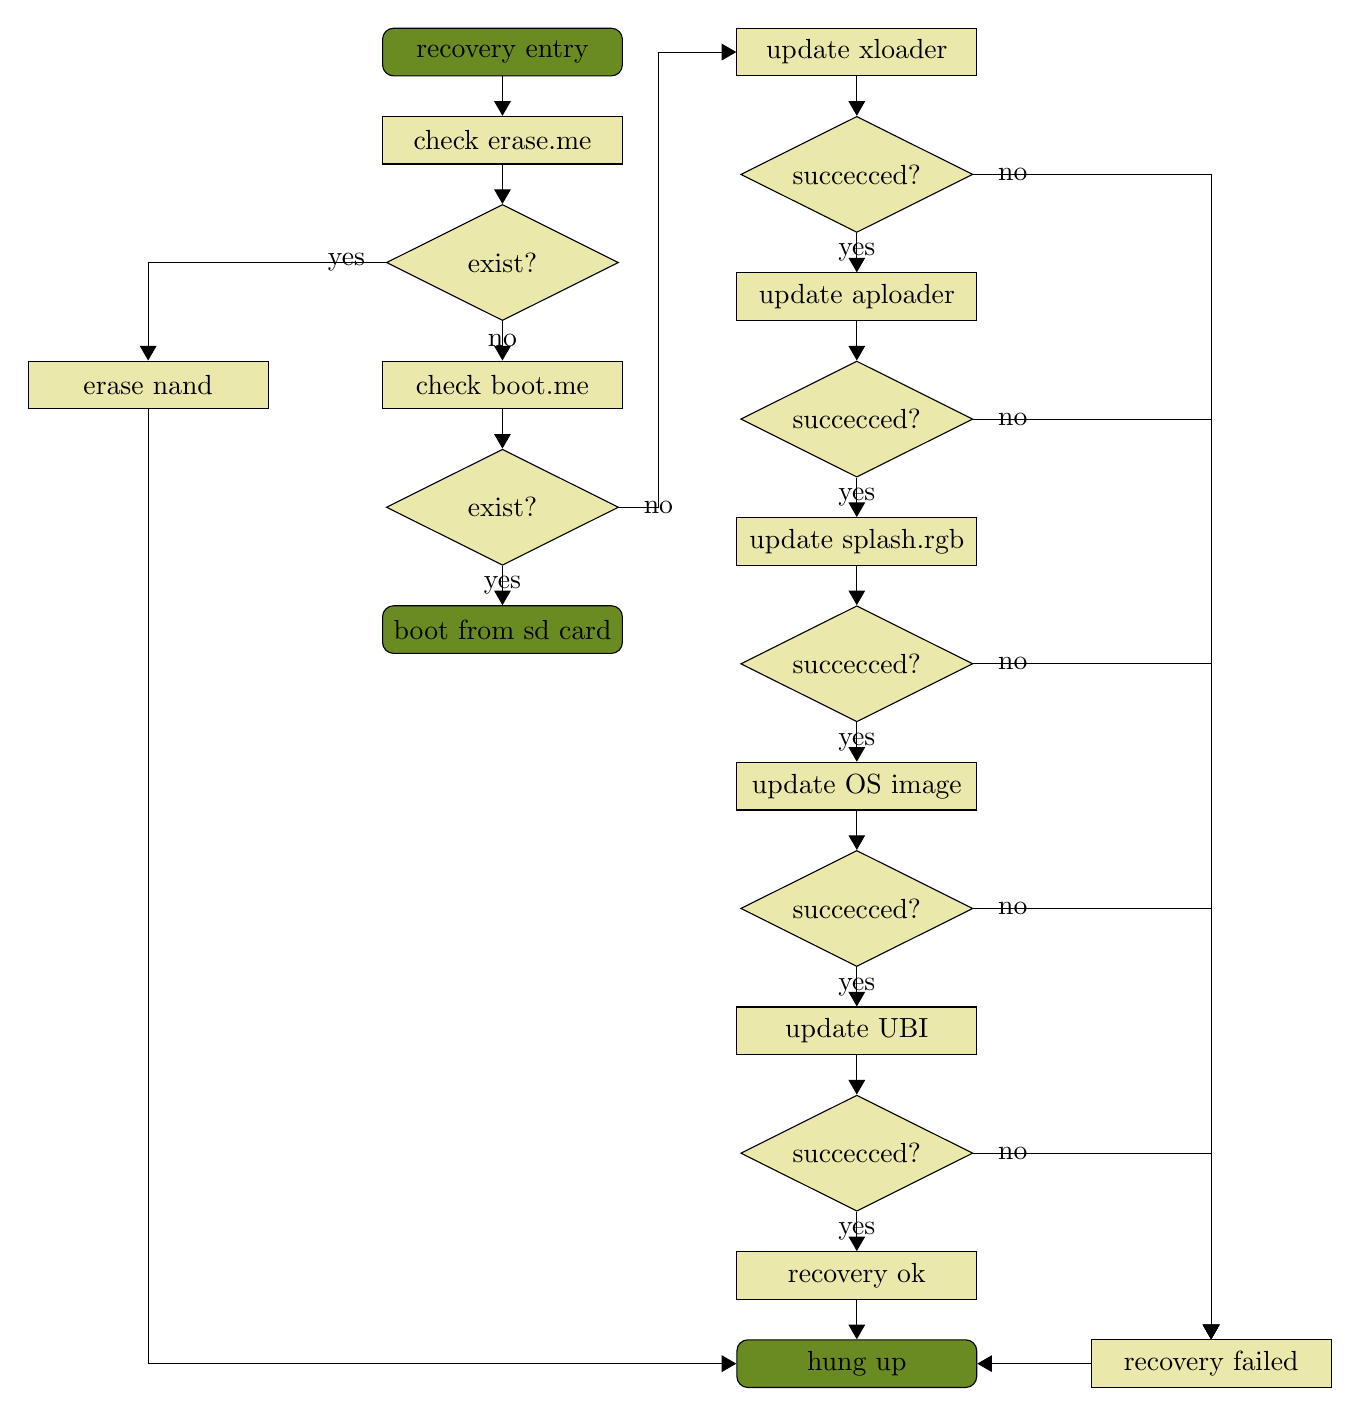
\begin{tikzpicture}[%
    >=triangle 60,              % Nice arrows; your taste may be different
    start chain=going below,    % General flow is top-to-bottom
    node distance=5mm and 45mm, % Global setup of box spacing
    every join/.style={norm},   % Default linetype for connecting boxes
    ]
\tikzset{
  base/.style={draw, on chain, on grid, align=center, minimum height=4ex},
  proc/.style={base, rectangle, text width=8em, fill=elemcolor},
  test/.style={base, diamond, aspect=2, text width=5em, fill=elemcolor},
  term/.style={base, rectangle, text width=8em, rounded corners, fill=namecolor},
}

\node [term] (p0) {recovery entry};
\node [proc] (p1) {check erase.me};
\node [test] (p2) {exist?};
\node [proc] (p3) {check boot.me};
\node [test] (p4) {exist?};

\node [proc,right=of p0] (p5) {update xloader};
\node [test] (p6) {succecced?};
\node [proc] (p7) {update aploader};
\node [test] (p8) {succecced?};
\node [proc] (p9) {update splash.rgb};
\node [test] (p10) {succecced?};
\node [proc] (p11) {update OS image};
\node [test] (p12) {succecced?};
\node [proc] (p13) {update UBI};
\node [test] (p14) {succecced?};
\node [proc] (p15) {recovery ok};
\node [term] (p16) {hung up};
\node [proc,right=of p16] (p17) {recovery failed};

\node [proc,left=of p3] (p18) {erase nand};
\node [term,below=of p4.south] (p19) {boot from sd card};

%connect
\draw [->] (p0.south) -- (p1.north);
\draw [->] (p1.south) -- (p2.north);
\draw [->] (p2.south) -- node {no} (p3.north);
\draw [->] (p2.west) -- ++(left:5mm) node {yes} -| (p18.north);
\draw [->] (p3.south) -- (p4.north);
\draw [->] (p4.east) -- ++(right:5mm) node {no} |- (p5.west);

\draw [->] (p4.south) -- node {yes} (p19.north);

\draw [->] (p6.south) -- node {yes} (p7.north);
\draw [->] (p8.south) -- node {yes} (p9.north);
\draw [->] (p10.south) -- node {yes} (p11.north);
\draw [->] (p12.south) -- node {yes} (p13.north);
\draw [->] (p14.south) -- node {yes} (p15.north);
\draw [->] (p6.east) -- ++(right:5mm) node {no} -| (p17.north);
\draw [->] (p8.east) -- ++(right:5mm) node {no} -| (p17.north);
\draw [->] (p10.east) -- ++(right:5mm) node {no} -| (p17.north);
\draw [->] (p12.east) -- ++(right:5mm) node {no} -| (p17.north);
\draw [->] (p14.east) -- ++(right:5mm) node {no} -| (p17.north);
\draw [->] (p5.south) -- (p6.north);
\draw [->] (p7.south) -- (p8.north);
\draw [->] (p9.south) -- (p10.north);
\draw [->] (p11.south) -- (p12.north);
\draw [->] (p13.south) -- (p14.north);
\draw [->] (p15.south) -- (p16.north);
\draw [->] (p17.west) -- (p16.east);

\draw [->] (p18.south) |- (p16.west);

\end{tikzpicture}
\caption{recovery flow chart}
\end{center}
\end{figure}

	The recovery process must program all the compents to nand, include xL\_CPlus.bin,
	ApLoader.bin, splash.rgb, os image and ubi binary image for the filesystem. The
	layout of these compents has been discussed in chapter 2 and chapter 3. If one of 
	these compents program failed, we just hung up the CPU.

	For aploader and splash.rgb, we have several copies in nand, and each copy occupies
	one block. If we found a bad block when program the aploader or splash.rgb, we just
	skip this block and program the next block, thus, the copies for the compent will be
	one less.

	We must program the aploader, splash.rgb and os image to the nand with an image header
	as descript in chapter 3. Figure 6 is the flow chart for aploader and splash.rgb program.

\begin{figure}[H]
\begin{center}
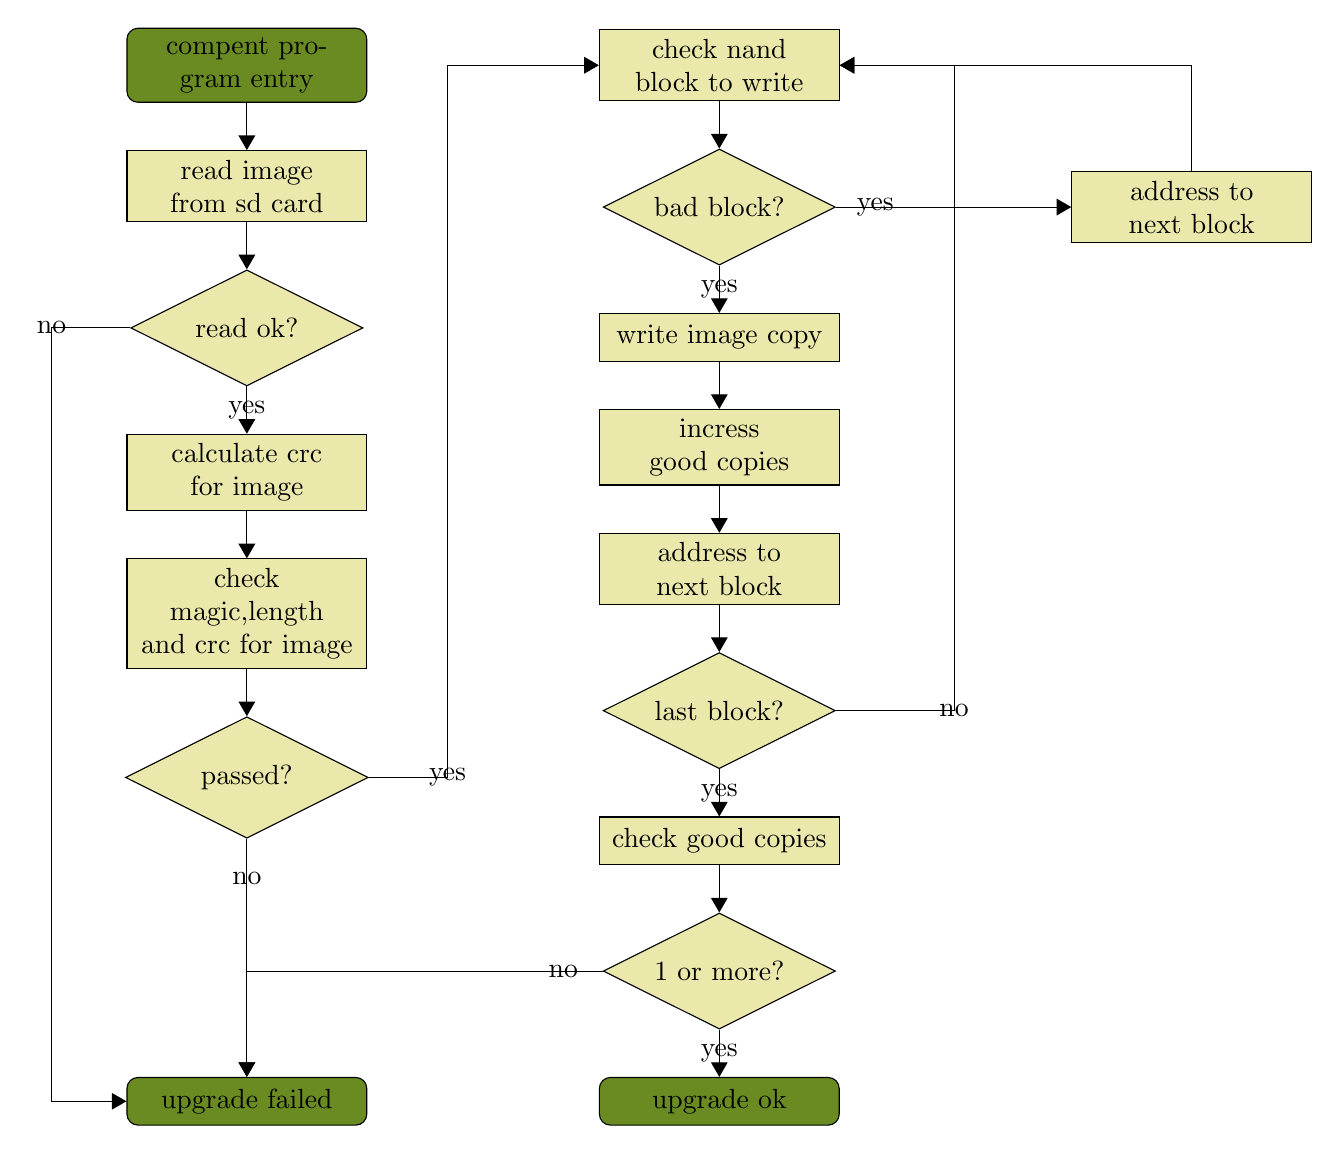
\begin{tikzpicture}[%
    >=triangle 60,              % Nice arrows; your taste may be different
    start chain=going below,    % General flow is top-to-bottom
    node distance=6mm and 60mm, % Global setup of box spacing
    every join/.style={norm},   % Default linetype for connecting boxes
    ]
\tikzset{
  base/.style={draw, on chain, on grid, align=center, minimum height=4ex},
  proc/.style={base, rectangle, text width=8em, fill=elemcolor},
  test/.style={base, diamond, aspect=2, text width=5em, fill=elemcolor},
  term/.style={base, rectangle, text width=8em, rounded corners, fill=namecolor},
}

\node [term] (p0) {compent program entry};
\node [proc] (p1) {read image from sd card};
\node [test] (p2) {read ok?};
\node [proc] (p3) {calculate crc for image};
\node [proc] (p4) {check magic,length and crc for image};
\node [test] (p5) {passed?};

\node [proc,right=of p0] (p6) {check nand block to write};
\node [test] (p7) {bad block?};
\node [proc,right=of p7] (p8) {address to next block};
\node [proc,below=of p7.south] (p9) {write image copy};
\node [proc] (p10) {incress good copies};
\node [proc] (p11) {address to next block};
\node [test] (p12) {last block?};
\node [proc] (p13) {check good copies};
\node [test] (p14) {1 or more?};
\node [term] (p15) {upgrade ok};
\node [term,left=of p15] (p16) {upgrade failed};

%connect
\draw [->] (p0.south) -- (p1.north);
\draw [->] (p1.south) -- (p2.north);
\draw [->] (p2.south) -- node {yes} (p3.north);
\draw [->] (p3.south) -- (p4.north);
\draw [->] (p4.south) -- (p5.north);

\draw [->] (p5.east) -- ++(right:10mm) node {yes} |- (p6.west);
\draw [->] (p6.south) -- (p7.north);
\draw [->] (p7.south) -- node {yes} (p9.north);
\draw [->] (p9.south) -- (p10.north);
\draw [->] (p10.south) -- (p11.north);
\draw [->] (p11.south) -- (p12.north);
\draw [->] (p12.south) -- node {yes} (p13.north);
\draw [->] (p13.south) -- (p14.north);
\draw [->] (p14.south) -- node {yes} (p15.north);

\draw [->] (p2.west) -- ++(left:10mm) node {no} |- (p16.west);
\draw [->] (p5.south) -- ++(down:5mm) node {no} -- (p16.north);
\draw [->] (p14.west) -- ++(left:5mm) node {no} -| (p16.north);

\draw [->] (p7.east) -- ++(right:5mm) node {yes} --  (p8.west);
\draw [->] (p8.north) |- (p6.east);
\draw [->] (p12.east) -- ++(right:15mm) node {no} |- (p6.east);

\end{tikzpicture}
\caption{ApLoader and splash.rgb program process}
\end{center}
\end{figure}

	For debug purpose, we need to boot up the os from the external sd card. If we found
	boot.me in the external sd card, we will try to load the ramfs and os image from the
	external sd card, and boot with these images. Figure 7 is the flow chart for boot
	from external sd card.

\begin{figure}[H]
\begin{center}
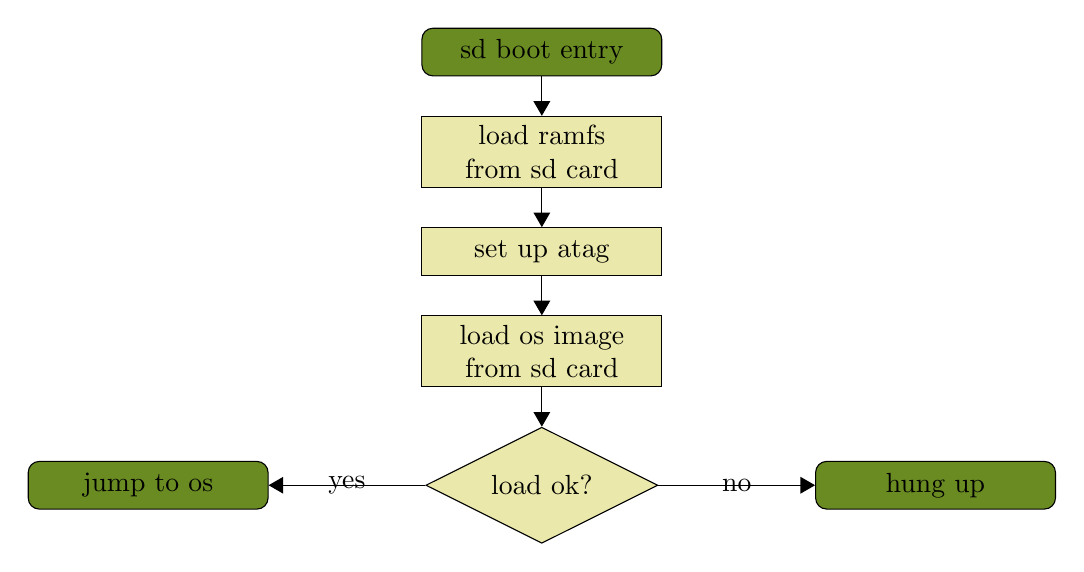
\begin{tikzpicture}[%
    >=triangle 60,              % Nice arrows; your taste may be different
    start chain=going below,    % General flow is top-to-bottom
    node distance=5mm and 50mm, % Global setup of box spacing
    every join/.style={norm},   % Default linetype for connecting boxes
    ]
\tikzset{
  base/.style={draw, on chain, on grid, align=center, minimum height=4ex},
  proc/.style={base, rectangle, text width=8em, fill=elemcolor},
  test/.style={base, diamond, aspect=2, text width=5em, fill=elemcolor},
  term/.style={base, rectangle, text width=8em, rounded corners, fill=namecolor},
}

\node [term] (p0) {sd boot entry};
\node [proc] (p1) {load ramfs from sd card};
\node [proc] (p2) {set up atag};
\node [proc] (p3) {load os image from sd card};
\node [test] (p4) {load ok?};
\node [term,left=of p4] (p5) {jump to os};
\node [term,right=of p4] (p6) {hung up};

\draw [->] (p0.south) -- (p1.north);
\draw [->] (p1.south) -- (p2.north);
\draw [->] (p2.south) -- (p3.north);
\draw [->] (p3.south) -- (p4.north);
\draw [->] (p4.east) -- node {no} (p6.west);
\draw [->] (p4.west) -- node {yes} (p5.east);

\end{tikzpicture}
\caption{boot from external sd card}
\end{center}
\end{figure}

\subsection{The boot process}
	At normal conditions, the aploader just load os image from nand and boot it. Figure
	8 is the flow chart of the normal boot progress.

\begin{figure}[H]
\begin{center}
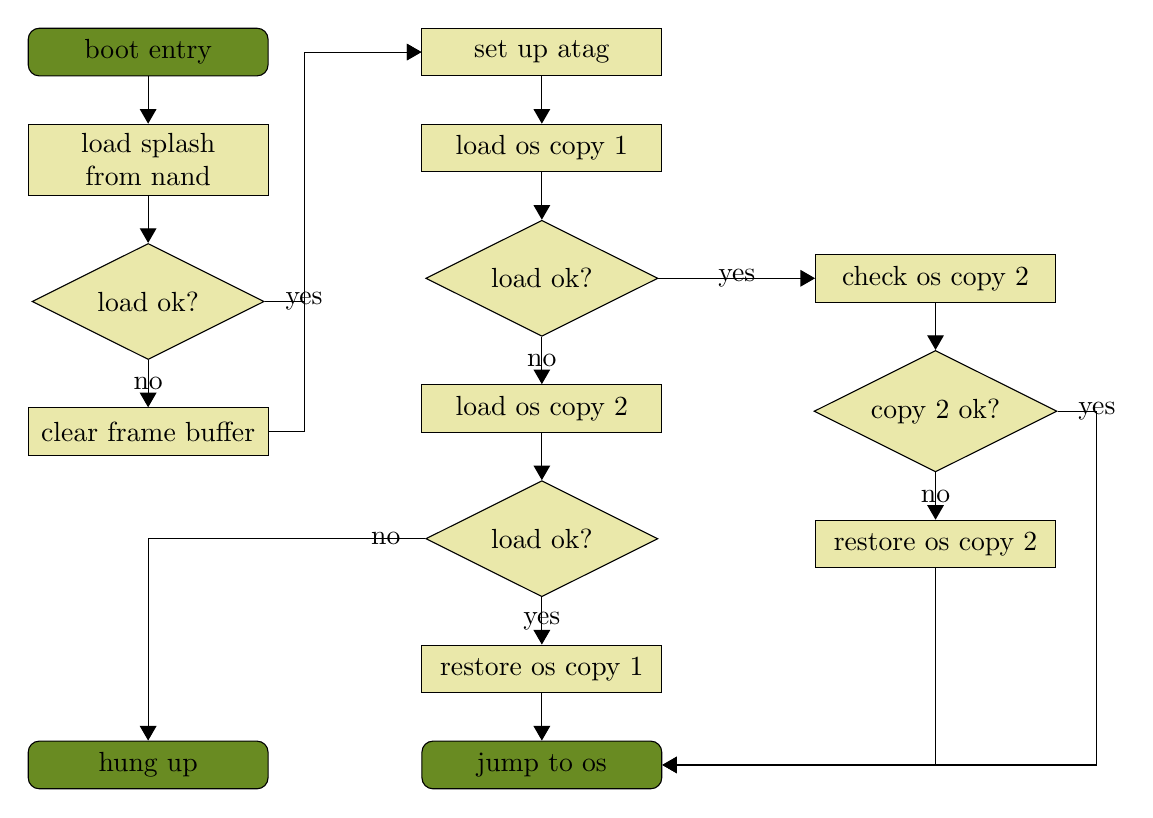
\begin{tikzpicture}[%
    >=triangle 60,              % Nice arrows; your taste may be different
    start chain=going below,    % General flow is top-to-bottom
    node distance=6mm and 50mm, % Global setup of box spacing
    every join/.style={norm},   % Default linetype for connecting boxes
    ]
\tikzset{
  base/.style={draw, on chain, on grid, align=center, minimum height=4ex},
  proc/.style={base, rectangle, text width=8em, fill=elemcolor},
  test/.style={base, diamond, aspect=2, text width=5em, fill=elemcolor},
  term/.style={base, rectangle, text width=8em, rounded corners, fill=namecolor},
}

\node [term] (p0) {boot entry};
\node [proc] (p1) {load splash from nand};
\node [test] (p2) {load ok?};
\node [proc] (p3) {clear frame buffer};

\node [proc,right=of p0] (p4) {set up atag};
\node [proc] (p5) {load os copy 1};
\node [test] (p6) {load ok?};
\node [proc] (p7) {load os copy 2};
\node [test] (p8) {load ok?};
\node [proc] (p9) {restore os copy 1};
\node [term] (p10) {jump to os};
\node [term,left=of p10] (p11) {hung up};

\node [proc,right=of p6] (p12) {check os copy 2};
\node [test] (p13) {copy 2 ok?};
\node [proc] (p14) {restore os copy 2};

%connect
\draw [->] (p0.south) -- (p1.north);
\draw [->] (p1.south) -- (p2.north);
\draw [->] (p2.south) -- node {no} (p3.north);
\draw [->] (p2.east) -- ++(right:5mm) node {yes} |- (p4.west);
\draw [->] (p3.east) -- ++(right:4.5mm) |- (p4.west);

\draw [->] (p4.south) -- (p5.north);
\draw [->] (p5.south) -- (p6.north);
\draw [->] (p6.south) -- node {no} (p7.north);
\draw [->] (p6.east) -- node {yes} (p12.west);
\draw [->] (p7.south) -- (p8.north);
\draw [->] (p8.south) -- node {yes} (p9.north);
\draw [->] (p8.west) -- ++(left:5mm) node {no} -| (p11.north);
\draw [->] (p9.south) -- (p10.north);
\draw [->] (p12.south) -- (p13.north);
\draw [->] (p13.south) -- node {no} (p14.north);
\draw [->] (p13.east) -- ++(right:5mm) node {yes} |- (p10.east);
\draw [->] (p14.south) |- (p10.east);

\end{tikzpicture}
\caption{boot from nand}
\end{center}
\end{figure}

	We must check the magic field, calculate the crc and compare with the origin written crc
	to decide if the image is ok or not. Please not that we do not restore the splash during
	boot, only check and restore the os image area.

	We have 4 copies of splash in nand. During boot, we start from the first one, if get a 
	good copy, then do not check the rest copies; If or the copies are bad, we get failed
	when load splash. It is the same with the ApLoader loading, which is done by the xLoader.

	Figure 9 is the flow chart for loading ApLoader and splash.

\begin{figure}[H]
\begin{center}
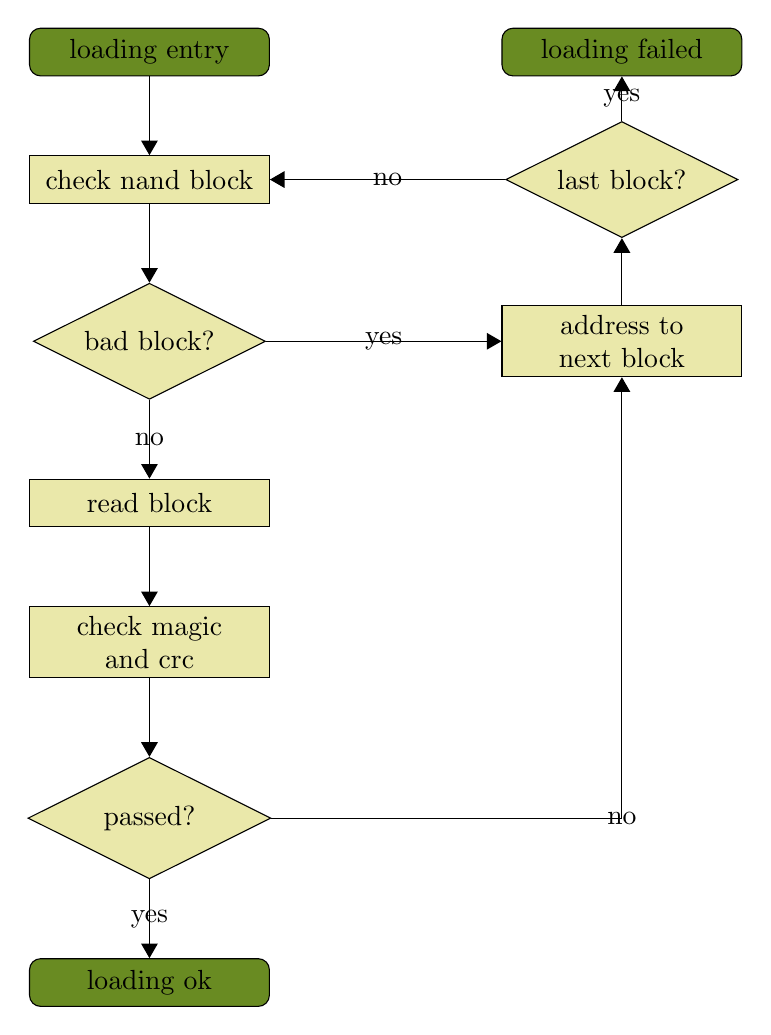
\begin{tikzpicture}[%
    >=triangle 60,              % Nice arrows; your taste may be different
    start chain=going below,    % General flow is top-to-bottom
    node distance=10mm and 60mm, % Global setup of box spacing
    every join/.style={norm},   % Default linetype for connecting boxes
    ]
\tikzset{
  base/.style={draw, on chain, on grid, align=center, minimum height=4ex},
  proc/.style={base, rectangle, text width=8em, fill=elemcolor},
  test/.style={base, diamond, aspect=2, text width=5em, fill=elemcolor},
  term/.style={base, rectangle, text width=8em, rounded corners, fill=namecolor},
}

\node [term] (p0) {loading entry};
\node [proc] (p1) {check nand block};
\node [test] (p2) {bad block?};
\node [proc] (p3) {read block};
\node [proc] (p4) {check magic and crc};
\node [test] (p5) {passed?};
\node [term] (p6) {loading ok};

\node [proc,right=of p2] (p7) {address to next block};
\node [test,right=of p1] (p8) {last block?};
\node [term,right=of p0] (p9) {loading failed};

%connect
\draw [->] (p0.south) -- (p1.north);
\draw [->] (p1.south) -- (p2.north);
\draw [->] (p2.south) -- node {no} (p3.north);
\draw [->] (p2.east) -- node {yes} (p7.west);
\draw [->] (p3.south) -- (p4.north);
\draw [->] (p4.south) -- (p5.north);
\draw [->] (p5.south) -- node {yes} (p6.north);
\draw [->] (p5.east) -| node {no} (p7.south);

\draw [->] (p7.north) -- (p8.south);
\draw [->] (p8.north) -- node {yes} (p9.south);
\draw [->] (p8.west) -- node {no} (p1.east);

\end{tikzpicture}
\caption{aploader and splash loading process}
\end{center}
\end{figure}

\section{DDR usage for aploader}
	We have total 128MiB DDR-II on the board, addressed from 0x00000000 to 0x08000000.
	Figure 10 is the layout of the DDR for aploader.

\begin{figure}[H]
\begin{center}

\newcommand{\memsection}[3]{
\node [draw,minimum height=#2*5mm,minimum width=6cm,fill=elemcolor] (#1) {#3};\\}

\newcommand{\freesection}[1]{
\node [draw,tape,tape bend top=none,minimum height=1cm,minimum width=6cm,fill=elemcolor] {#1};\\
\node [draw,tape,tape bend bottom=none,minimum height=1cm,minimum width=6cm,fill=elemcolor] {#1};\\}

\begin{tikzpicture}[node distance=0mm and 10mm]
	\matrix (mainmemory) [row sep=-\pgflinewidth]
	{
		\memsection{framebuffer} {1} {frame buffer}
		\freesection{free}
		\memsection{sgafb} {1} {display buffer}
		\memsection{sgabuf} {1} {internal buffer}
		\memsection{sgabt} {1} {command batch}
		\memsection{sgafw} {1} {firmware}
		\freesection{free}
		\memsection{aploader} {4} {aploader code \& stack}
		\freesection{free}
		\memsection{ramfs} {8} {init ramfs}
		\memsection{osimage} {6} {os image \& param}
	};

	\node [left=of osimage.south west,align=right,text width=4cm] (bottom) {0x0000 0000};
	\node [above=0mm of bottom, align=right,text width=4cm] (osparam) {os param/0x0000 0100};
	\node [above=1mm of osparam, align=right,text width=4cm] (osentry) {os entry/0x0000 8000};
	\node [left=of ramfs.south west,align=right,text width=4cm] (ramfsentry) {init ramfs/0x0080 0000};
	\node [left=of aploader.south west,align=right,text width=4cm] (alentry) {code/0x03e0 0000};
	\node [left=of aploader.north west,align=right,text width=4cm] (alend) {stack/0x03f0 0000};
	\node [left=of aploader.west,align=right,text width=4cm] (alheapd) {heap start/0x03e8 0000};
	\node [above=-1.5mm of alheapd,align=right,text width=4cm] (alheapu) {heap end/0x03ea 0000};
	\node [left=of sgafw.south west,align=right,text width=4cm] (sgaentry) {0x06f0 0000};
	\node [left=of sgabt.south west,align=right,text width=4cm] (sgabtentry) {0x0700 0000};
	\node [left=of sgabuf.south west,align=right,text width=4cm] (sgabufentry) {0x0710 0000};
	\node [left=of sgafb.south west,align=right,text width=4cm] (sgafbentry) {0x0720 0000};
	\node [left=of sgafb.north west,align=right,text width=4cm] (sgafbend) {0x0730 0000};
	\node [left=of framebuffer.south west,align=right,text width=4cm] (fbentry) {0x07f0 0000};
	\node [left=of framebuffer.north west,align=right,text width=4cm] (fbend) {0x0800 0000};

	%connect
	\draw [->] (bottom) -- (osimage.south west);
	\draw [->] (osparam) -- (osimage.197);
	\draw [->] (osentry) -- (osimage.183);
	\draw [->] (ramfsentry) -- (ramfs.south west);
	\draw [->] (alentry) -- (aploader.south west);
	\draw [->] (alend) -- (aploader.north west);
	\draw [->] (alheapd) -- (aploader.west);
	\draw [->] (alheapu) -- (aploader.170);
	\draw [->] (sgaentry) -- (sgafw.south west);
	\draw [->] (sgabtentry) -- (sgabt.south west);
	\draw [->] (sgabufentry) -- (sgabuf.south west);
	\draw [->] (sgafbentry) -- (sgafb.south west);
	\draw [->] (sgafbend) -- (sgafb.north west);
	\draw [->] (fbentry) -- (framebuffer.south west);
	\draw [->] (fbend) -- (framebuffer.north west);

\end{tikzpicture}

\caption{DDR usage for aploader}
\end{center}
\end{figure}

\end{document}
